\section{Metodologia}

\subsection{Modulação AM-DSB-SC (Double Sideband Suppressed Carrier)}

Neste experimento, utilizou-se o GNU Radio Companion (GRC) para implementar a modulação AM-DSB-SC. O sinal de mensagem foi gerado utilizando um bloco de fonte de sinal senoidal com frequência $f_{m}$ de 1 kHz e amplitude de 1. A portadora foi gerada com frequência de 5 kHz e amplitude de 1. O sinal modulado foi obtido multiplicando o sinal de mensagem pela portadora.

O diagrama de blocos da modulação AM-DSB-SC no GNU Radio é apresentado na Figura \ref{fig:modulacao_am_sc}.

\begin{figure}
    \centering
    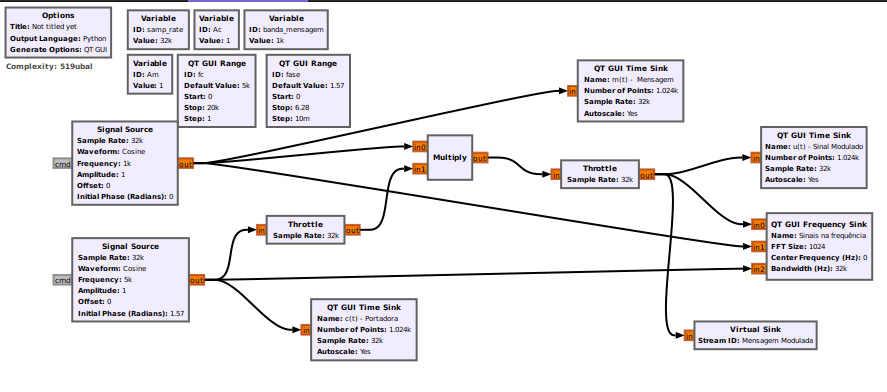
\includegraphics[width=0.5\textwidth]{images/mod_am_sc_gnu.png}
    \caption{Diagrama de blocos da modulação AM-DSB-SC. Fonte: Autor.}
    \label{fig:modulacao_am_sc}
\end{figure}

Os seguintes blocos foram utilizados:

\begin{itemize}
    \item \textbf{Signal Source}: Gera o sinal de mensagem com frequência de 1000 Hz e amplitude de 1.
    \item \textbf{Signal Source}: Gera a portadora com frequência variável de 0 a 20 kHz e amplitude de 1 V.
    \item \textbf{Signal Source}: Gera o oscilador local com frequência fixa de 5 kHz.
    \item \textbf{QT GUI Range}: Permite ajustar a frequência da portadora entre 0 e 20 kHz.
    \item \textbf{Multiply}: Multiplica o sinal de mensagem pela portadora, resultando no sinal modulado AM-DSB-SC.
    \item \textbf{Virtual Sink}: Armazena os sinais para uso no bloco Virtual Source.
    \item \textbf{Virtual Source}: Utiliza os sinais armazenados no bloco Virtual Sink.
    \item \textbf{QT GUI Time Sink}: Exibe o sinal modulado no domínio do tempo.
    \item \textbf{QT GUI Frequency Sink}: Exibe o espectro do sinal modulado no domínio da frequência.
\end{itemize}

Para demonstrar a perda da mensagem devido à falta de sincronismo, ajustou-se a frequência da portadora para 10 kHz e modificou-se a fase do sinal para 1,57 radianos (90°) através do QT GUI Range. Com esses valores, espera-se que na demodulação a mensagem seja completamente comprometida.

\subsection{Demodulação AM-DSB-SC (Double Sideband Suppressed Carrier)}

Implementou-se a demodulação do sinal AM-DSB-SC multiplicando o sinal modulado por um oscilador local com a mesma frequência e fase da portadora original, seguido de um filtro passa-baixas.

O diagrama de blocos da demodulação AM-DSB-SC no GNU Radio é apresentado na Figura \ref{fig:demodulacao_am_sc_gnu}.

\begin{figure}
    \centering
    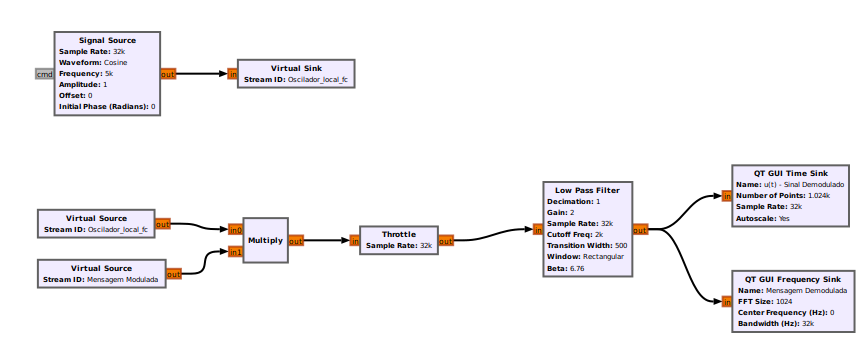
\includegraphics[width=0.5\textwidth]{images/demodulacao_gnu_am_dscb_sc.png}
    \caption{Diagrama de blocos da demodulação AM-DSB-SC. Fonte: Autor.}
    \label{fig:demodulacao_am_sc_gnu}
\end{figure}

Os blocos utilizados foram:

\begin{itemize}
    \item \textbf{Virtual Source}: Recebe o sinal modulado armazenado.
    \item \textbf{Signal Source}: Gera o oscilador local com frequência igual à portadora (5 kHz).
    \item \textbf{Multiply}: Multiplica o sinal modulado pelo oscilador local.
    \item \textbf{Throttle}: Controla a taxa de amostragem.
    \item \textbf{Low Pass Filter}: Filtro passa-baixas com frequência de corte em 2 kHz, ganho de 2 e janela retangular.
    \item \textbf{QT GUI Time Sink}: Exibe o sinal demodulado no tempo.
    \item \textbf{QT GUI Frequency Sink}: Exibe o espectro demodulado.
\end{itemize}

Para demonstrar a importância do sincronismo, utilizou-se uma portadora com frequência diferente da do oscilador local no receptor.

\subsection{Modulação AM Convencional}

Para gerar o sinal AM convencional, adicionou-se uma constante ao sinal de mensagem antes da multiplicação pela portadora. Mantiveram-se os controles de frequência para demonstrar a insensibilidade à fase na demodulação por detector de envoltória.

Os parâmetros e blocos utilizados foram:

\begin{itemize}
    \item \textbf{Signal Source}: Gera o sinal de mensagem (1 kHz, amplitude 1).
    \item \textbf{QT GUI Range}: Ajusta a frequência da portadora (50 Hz a 20 kHz).
    \item \textbf{Add}: Soma uma constante DC de 1 ao sinal de mensagem.
    \item \textbf{Multiply}: Multiplica pelo sinal da portadora.
    \item \textbf{Multiply Const}: Ajusta a amplitude do sinal mensagem (500 mV).
    \item \textbf{Virtual Sink/Source}: Armazena e recupera os sinais.
    \item \textbf{Throttle}: Controla a taxa de amostragem.
    \item \textbf{QT GUI Time/Frequency Sink}: Visualização dos sinais.
\end{itemize}

O diagrama de blocos é mostrado na Figura \ref{fig:modulacao_am_gnu}.

\begin{figure}
    \centering
    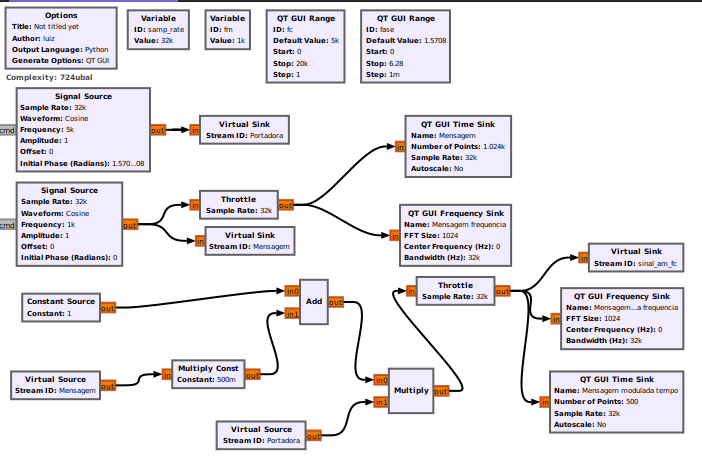
\includegraphics[width=0.5\textwidth]{images/convecional_gnu.png}
    \caption{Diagrama de blocos da modulação AM convencional. Fonte: Autor.}
    \label{fig:modulacao_am_gnu}
\end{figure}

\subsection{Demodulação AM Convencional}

A demodulação por detector de envoltória foi implementada conforme a Figura \ref{fig:demodulacao_am_gnu}, utilizando:

\begin{itemize}
    \item \textbf{Virtual Source}: Recebe o sinal modulado.
    \item \textbf{Low Pass Filter}: Filtra o sinal demodulado.
    \item \textbf{Python Block} (Retificador): Implementa a retificação de meia-onda.
    \item \textbf{DC BlockR}: Remove a componente DC.
    \item \textbf{QT GUI Time/Frequency Sink}: Visualização dos resultados.
\end{itemize}


\subsubsection*{Implementação em GNU Radio: Retificador de Meia Onda}

A seguir, apresenta-se uma implementação em Python de um bloco de retificação de meia onda para sinais reais, utilizando GNU Radio:

\begin{lstlisting}[language=Python, caption={Implementação do retificador de meia onda}]
import numpy as np
from gnuradio import gr

class blk(gr.sync_block):
    """Retificador de meia onda (sinal real)"""

    def __init__(self):
        gr.sync_block.__init__(
            self,
            name='Retificador Meia Onda',
            in_sig=[np.float32],
            out_sig=[np.float32]
        )

    def work(self, input_items, output_items):
        # zera os valores negativos
        output_items[0][:] = np.maximum(input_items[0], 0)
        return len(output_items[0])
\end{lstlisting}


\begin{figure}
    \centering
    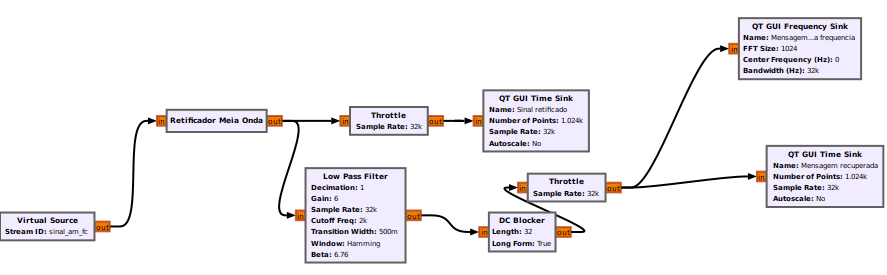
\includegraphics[width=0.5\textwidth]{images/demodulcao_am_convencional_gnu.png}
    \caption{Diagrama de blocos da demodulação AM convencional. Fonte: Autor.}
    \label{fig:demodulacao_am_gnu}
\end{figure}

\subsection{Efeitos da Fase na Demodulação AM Convencional}

Ao contrário da modulação DSB-SC, na demodulação AM convencional por detector de envoltória:
\begin{itemize}
    \item A fase da portadora \textbf{não afeta} a demodulação, pois o detector extrai apenas a envoltória do sinal.
    \item Mesmo com variações de fase na portadora, a mensagem é recuperada sem distorção.
    \item O detector é insensível à frequência exata da portadora, desde que esta seja suficientemente alta em relação à largura de banda do sinal modulante.
\end{itemize}

Para demonstrar essa característica:
\begin{itemize}
    \item Variou-se a fase da portadora através do QT GUI Range.
    \item Ajustou-se a frequência da portadora para valores diferentes da original.
    \item Observou-se que a mensagem demodulada mantém sua forma de onda independentemente desses parâmetros.
\end{itemize}

Esta insensibilidade à fase comprova a vantagem do detector de envoltória em aplicações onde o sincronismo preciso não é viável.